\documentclass[runningheads]{llncs}
% PROVISIONAL: official Springer LLNCS class v2.26 (CTAN mirror of Springer's llncs package). Generated by build_main.py.
% (no T1 fontenc: avoids bitmap font generation)
\AtBeginDocument{\pdfpagewidth=210mm \pdfpageheight=297mm} % A4 PDF; llncs fixes only the 12.2x19.3 cm text block
\usepackage{graphicx}
\usepackage{booktabs}
\usepackage{amsmath,amssymb}
\usepackage{algorithm}
\usepackage{algpseudocode}
\usepackage{url}
\usepackage{array}
\setcounter{topnumber}{3}\setcounter{totalnumber}{5}\renewcommand{\topfraction}{0.9}\renewcommand{\bottomfraction}{0.8}\renewcommand{\textfraction}{0.1}\renewcommand{\floatpagefraction}{0.75}
\begin{document}
\title{Does Dimensionality Reduction Help Classical Intrusion Detection? Original Features versus PCA and Kernel PCA on a Class-Stratified CIC-IDS2017 Sample}
\titlerunning{~}
\ifdefined\BLIND
\author{Anonymous Author(s)}
\authorrunning{~}
\institute{Anonymous Institution}
\else
\author{}
\authorrunning{~}
\institute{}
\fi
\maketitle
\begin{abstract}
Kernel principal component analysis (KPCA) is often paired with classical classifiers for network intrusion detection, but gains are sometimes reported on a single split or without a no-reduction baseline. We compare the 78 original CIC-IDS2017 flow features with PCA and KPCA (linear, RBF and cosine kernels; 5 to 30 components) across five classifiers: logistic regression, $k$-nearest neighbors, SVM, decision tree and random forest. The data are a class-stratified sample of 6,000 records (at least 100 per class) drawn after exact duplicate removal; the sample does not preserve natural traffic prevalence. Imputation, scaling and reduction are fitted on training folds only. Evaluation combines repeated stratified cross-validation, nested cross-validation, a small nested hyper-parameter search, two row-order checks that serve as an unverified proxy for chronology (the files contain no timestamps), and a runtime and memory benchmark. A random forest on the original features scored highest (macro-F1 $0.901\pm0.020$; accuracy $0.972\pm0.004$; nested estimate $0.900\pm0.022$), yet two web-attack classes had F1 of only 0.53 and 0.59. Reduction did not help the decision tree or random forest and at best matched the original features for logistic regression and $k$-NN. Only the SVM gained from reduction (cosine KPCA), and that gain fell from 0.076 to 0.021 after tuning. In our benchmark, KPCA fitting took more than 200 times longer than PCA and whole-pipeline traced memory was about 37 times higher. The results come from one sample of one dataset, and every significance test carries a fold-dependence caveat.

\keywords{Network intrusion detection \and CIC-IDS2017 \and Kernel PCA \and Dimensionality reduction \and Class imbalance \and Machine learning.}
\vspace{2pt}\noindent\textit{Code and results:} \ifdefined\BLIND link withheld for anonymous review\else[REPOSITORY URL / ARCHIVE DOI -- TO BE FILLED BY THE AUTHORS]\fi
\end{abstract}

\section{Introduction}
Network intrusion detection systems (NIDS) are usually developed and compared on public flow datasets \cite{ring2019}, and CIC-IDS2017 \cite{sharafaldin2018} is widely used for this. Its MachineLearningCVE files describe each flow with 78 numeric features, which makes dimensionality reduction tempting, either to cut training cost or in the hope of better generalization. Linear PCA and auto-encoders have been tried on CIC-IDS2017 \cite{abdulhammed2019}. Kernel PCA (KPCA) \cite{scholkopf1998} runs PCA in an implicit nonlinear feature space and has been paired with SVMs for intrusion detection \cite{kuang2014}.

Three problems make such comparisons hard to interpret. First, CIC-IDS2017 is imbalanced and, in its original form, contains labelling and flow-construction errors \cite{engelen2021,panigrahi2018}, so the benign majority can dominate accuracy. Second, machine learning for security is prone to pitfalls that inflate results \cite{arp2022}. Third, a claim that reduction helps means little without a no-reduction baseline; otherwise the benefit is assumed rather than measured.

\textbf{Research questions.} \textbf{RQ1:} how does reduction change multi-class detection performance? \textbf{RQ2:} does KPCA beat the original space or ordinary PCA? \textbf{RQ3:} how do kernel, number of components and classifier interact? \textbf{RQ4:} what does reduction cost in time and memory? \textbf{RQ5:} do the conclusions hold under repeated class-aware validation, nested selection, tuning and row-order splits (a proxy for chronology)?

\textbf{Contributions.} (i) A reproducible comparison of the original features, PCA and three KPCA kernels over five classical classifiers, on a sample taken from the raw files after exact same-label duplicate removal. It uses fold-wise fitting, a majority-class baseline, a nested-CV check of selection optimism and a small nested hyper-parameter search. (ii) A class-aware analysis of how far accuracy overstates detection quality. (iii) Paired statistical tests with an explicit independence caveat, plus two row-order robustness checks (proxy chronology). (iv) A runtime and memory comparison of KPCA with PCA. We propose no new algorithm. Code and results are described in the Data and Code Availability section.

\section{Related Work}
We surveyed fifteen studies. Table~\ref{tab:lit} lists five recent (2025) ones with algorithm, dataset and result \emph{as stated by their authors}; the other ten, on the dataset and its problems, dimensionality reduction and evaluation practice, are discussed below.


\textit{Dataset and its quality.} \textbf{Ring et al.}~\cite{ring2019} survey public network-intrusion datasets and define 15 properties for judging which evaluation settings each dataset suits; we cite it for the criteria by which flow datasets are judged. \textbf{Sharafaldin et al.}~\cite{sharafaldin2018} introduced CIC-IDS2017 and describe its traffic and attack scenarios; we use the original flow files they distribute. \textbf{Engelen et al.}~\cite{engelen2021} report ``TCP appendix'' artefact flows (about a quarter of all flows), attack attempts labelled as attacks although they contain no malicious payload, and feature-extraction flaws that enable shortcut learning, and they released a corrected version; this limits how far our absolute scores can be trusted. \textbf{Panigrahi and Borah}~\cite{panigrahi2018} likewise describe shortcomings of the dataset and propose a combined dataset, which we did not use. Together these four papers bear on how far CIC-IDS2017 scores can be trusted; none studies dimensionality reduction.

\textit{Dimensionality reduction.} \textbf{Abdulhammed et al.}~\cite{abdulhammed2019} apply an auto-encoder and PCA to CIC-IDS2017, reducing 81 features to 10 and reporting about 99.6\,\% accuracy in multi-class and binary classification; they are our nearest CIC-IDS2017 reference for PCA. \textbf{Kuang et al.}~\cite{kuang2014} combine KPCA, an SVM and a genetic algorithm for intrusion detection; this is a related earlier KPCA--SVM approach, but it predates CIC-IDS2017 and therefore could not have evaluated that dataset. \textbf{Abdel-Rahman et al.}~\cite{abdelrahman2026} propose a feature-importance-guided autoencoder and state that, with a random forest, it outperformed earlier reduction techniques on NSL-KDD, UNSW-NB15 and CIC-IDS2017; we did not extract their numbers, and we study classical reducers rather than a learned one. \textbf{Chavan and Alone}~\cite{chavan2025} report ``high accuracy'' for a random forest on CIC-IDS 2017, with no figure or split in the abstract, so there is nothing to compare numerically with our random-forest result.

\textit{Evaluation methodology.} \textbf{Arp et al.}~\cite{arp2022} describe pitfalls in machine learning for security that can produce unrealistic performance; in response we fit every data-dependent step on training folds only and report class-aware metrics beside accuracy. \textbf{Apruzzese et al.}~\cite{apruzzese2022} propose cross-evaluating ML-based network intrusion detection across datasets; we do not, so our conclusions stay within one dataset. Among the studies we read, none pairs a no-reduction baseline, per-class analysis and fold-wise fitting across PCA and several KPCA kernels. Our reading was not exhaustive, so this is not a claim about a gap in the literature. IEEE Xplore was not accessible during our search; we used publisher records, proceedings, repositories and preprints.

\begin{table}[htbp]
\caption{Recent studies (2025) and this work. Results are quoted from each source and are not directly comparable (different datasets, sampling, splits and metrics).}\label{tab:lit}
\centering\scriptsize
\renewcommand{\arraystretch}{1.15}
\begin{tabular}{@{}>{\raggedright\arraybackslash}p{2.3cm}>{\raggedright\arraybackslash}p{3.3cm}>{\raggedright\arraybackslash}p{2.4cm}>{\raggedright\arraybackslash}p{1.7cm}>{\raggedright\arraybackslash}p{1.7cm}@{}}
\toprule
Author (year) & Title & Algorithm & Dataset & Reported result \\
\midrule
Waghmode et al.\ \cite{waghmode2025} (2025) & Intrusion detection system based on machine learning using least square support vector machine & Quantum-inspired LS-SVM with exhaustive feature selection & NSL-KDD, CIC-IDS-2017, UNSW-NB15 & Accuracy 99.5\,\% on CIC-IDS-2017 \\
Patil et al.\ \cite{patil2025} (2025) & Optimizing network intrusion detection systems through ensemble learning and feature selection using the CIC-IDS2017 dataset & Bagging and boosting ensembles; information gain, chi-square, PCA-based feature selection (20 features) & CIC-IDS2017, stratified 70/30 split & Accuracy 99.98\,\% (Extra Trees, 24 features); 99.58--99.96\,\% with PCA-based selection \\
Abdelaziz et al.\ \cite{abdelaziz2025} (2025) & Enhancing network threat detection with random forest-based NIDS and permutation feature importance & Random forest, permutation importance, undersampling; repeated stratified 5-fold CV & CIC-IDS2017 & Weighted-F1 99.8\,\%, macro-F1 93.31\,\% (26 features) \\
Xu and Liu \cite{xu2025} (2025) & Robust anomaly detection in network traffic: evaluating machine learning models on CICIDS2017 & MLP, 1D-CNN, one-class SVM, LOF & CICIDS2017 & Accuracy 97.75\,\% (MLP, overall test set) \\
Emirmahmuto\u{g}lu and Atay \cite{emirmahmutoglu2025} (2025) & A feature selection-driven machine learning framework for anomaly-based intrusion detection systems & PSO/FPA/DE feature selection; LR, DT, RF, k-NN and others & KDD CUP 99, NSL-KDD, UNSW-NB15, CSE-CIC-IDS2018 & 99.987\,\% (results) / 99.9965\,\% (conclusion); source inconsistent (FPA, RF) \\
\midrule
\textbf{This work} (2026) & (this paper) & Original features vs PCA vs linear/RBF/cosine KPCA; LR, k-NN, SVM, DT, RF & CIC-IDS2017, 6,000-record class-stratified sample & RF (original): accuracy 97.2\,\%, macro-F1 90.1\,\% \\
\bottomrule
\end{tabular}
\end{table}

\section{Dataset and Preprocessing}\label{sec:data}
\textbf{Data.} We use the eight daily CIC-IDS2017 \texttt{MachineLearningCVE} files: 2{,}830{,}743 flows, 78 numeric features, 15 labels (counts computed from the files; no provider checksum was available). There is no timestamp column. Rows with missing or infinite values are 0.2\,\% or less of each file (inf $\to$ NaN) and were not imputed before sampling. Eight features are constant in every file and were kept to match the 78-feature definition of earlier work.

\textbf{Duplicates.} 308{,}381 flows (10.9\,\%) are exact duplicates (identical on all 78 features and the label) of another flow and were removed before sampling, because identical flows in training and test folds inflate scores. Feature-identical flows with \emph{different} labels were not removed: 698 such conflicting-label groups remain in the 2.52\,M pool. None of them fell into the 6{,}000-record sample: it contains no two records with identical feature vectors, with the same or with different labels. Duplication is uneven: removal took 43\,\% of PortScan flows (158{,}930 to 90{,}819) and 25\,\% of DoS Hulk flows, versus 7.8\,\% of benign flows.

\textbf{Sample.} Exact KPCA needs an $n\times n$ kernel matrix, so we draw a stratified random sample of 6{,}000 records from the de-duplicated pool of 2{,}522{,}362 flows (seed 0): each class contributes at least 100 records (all of them if fewer exist) and the rest is allocated proportionally to pool prevalence. Heartbleed (11), SQL injection (21) and Infiltration (36) are therefore complete but tiny; the floor over-represents attack classes relative to real traffic (benign: 67.2\,\% of the sample versus 83\,\% of the pool). Sampling uses only labels and random numbers; \emph{no imputation or scaling statistic is computed before the split}. Only two feature cells in the sample are missing; they are imputed with training-fold means inside each fold. Each record keeps its source file (day) and row position for the row-order checks.



\section{Methodology}\label{sec:method}
\textbf{Pipeline.} Fig.~\ref{fig:pipe} shows the protocol. Within each training fold we fit a mean imputer and a standard scaler, then the dimensionality reducer; test folds are only transformed. Feature spaces are: \emph{original} (78 standardised features); \emph{PCA}; and \emph{KPCA} with linear, RBF (scikit-learn default $\gamma=1/78$) and cosine kernels \cite{scholkopf1998}, each with $n\in\{5,10,15,20,30\}$ components. The reducer is fitted once per fold and shared by all classifiers, which is equivalent to fitting it inside each pipeline because it is deterministic (unit-tested).

\begin{figure}[htbp]\centering
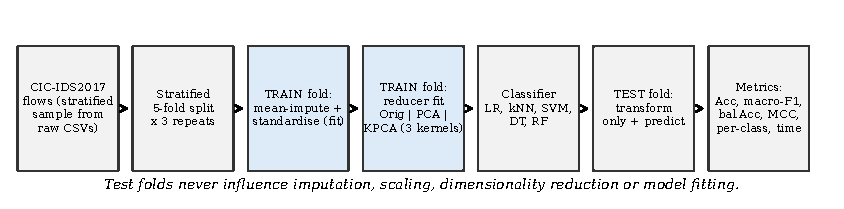
\includegraphics[width=\textwidth]{figures/fig1_pipeline.pdf}
\caption{Experimental pipeline. All data-dependent preprocessing and reduction is fitted on the training fold only.}\label{fig:pipe}
\end{figure}

\textbf{Algorithm and formulas.} Algorithm~\ref{alg:cv} summarises one evaluation of a feature space and classifier. Features are standardised as $z_j=(x_j-\mu_j)/\sigma_j$ with $\mu_j,\sigma_j$ from the training fold. PCA projects onto the leading eigenvectors $\mathbf{v}_k$ of the training covariance matrix $\mathbf{C}=\frac{1}{n}\mathbf{Z}^{\top}\mathbf{Z}$. KPCA uses the kernel matrix $K_{ij}=k(\mathbf{z}_i,\mathbf{z}_j)$ with
\begin{equation}
k_{\mathrm{lin}}=\mathbf{z}^{\top}\mathbf{z}',\qquad k_{\mathrm{rbf}}=\exp(-\gamma\lVert\mathbf{z}-\mathbf{z}'\rVert^{2}),\ \gamma=\tfrac{1}{78},\qquad k_{\cos}=\frac{\mathbf{z}^{\top}\mathbf{z}'}{\lVert\mathbf{z}\rVert\,\lVert\mathbf{z}'\rVert},
\end{equation}
centred as $\tilde{K}=K-\mathbf{1}_nK-K\mathbf{1}_n+\mathbf{1}_nK\mathbf{1}_n$; with $\mathbf{1}_n$ the $n\times n$ matrix whose entries are all $1/n$. For the leading eigenpairs $(\lambda_k,\boldsymbol{\alpha}_k)$ of $\tilde{K}$, with $\lVert\boldsymbol{\alpha}_k\rVert=1$, a sample is projected to $\tilde{K}_{\mathrm{new}}\boldsymbol{\alpha}_k/\sqrt{\lambda_k}$, with $\tilde{K}_{\mathrm{new}}$ the centred kernel against the training fold (matches \texttt{KernelPCA.transform}; dividing by $\lambda_k$ does not). With per-class precision $P_c$ and recall $R_c$, the primary metric is
\begin{equation}
F1_c=\frac{2P_cR_c}{P_c+R_c},\qquad \text{macro-F1}=\frac{1}{C}\sum_{c=1}^{C}F1_c,\ \ C=15,
\end{equation}
and balanced accuracy equals macro-recall. The multi-class MCC from the confusion matrix $\mathbf{M}$ with $s$ samples, $t_k$ true and $p_k$ predicted counts of class $k$, and $c=\sum_k M_{kk}$ correct predictions is
\begin{equation}
\mathrm{MCC}=\frac{c\,s-\sum_k p_kt_k}{\sqrt{s^{2}-\sum_k p_k^{2}}\,\sqrt{s^{2}-\sum_k t_k^{2}}}.
\end{equation}

\begin{algorithm}[t]
\caption{Fold-wise evaluation of one feature space $S$ and classifier $f$}\label{alg:cv}
\begin{algorithmic}[1]
\Require sample $(X,y)$ of 6,000 records; space $S\in\{$original, PCA, KPCA$(k,n)\}$; classifier $f$; 3 repeats of stratified 5-fold CV (seed 42)
\Ensure mean and standard deviation of accuracy, macro-F1, MCC and cost over 15 folds
\For{each repeat $r$ and fold $(\mathrm{tr},\mathrm{te})$}
  \State fit mean imputer and standard scaler on $X_{\mathrm{tr}}$; transform $X_{\mathrm{tr}}$ and $X_{\mathrm{te}}$
  \If{$S\neq$ original}
    \State fit reducer $T_S$ ($n$ components) on the scaled $X_{\mathrm{tr}}$ only
    \State $Z_{\mathrm{tr}}\gets T_S(X_{\mathrm{tr}})$;\ $Z_{\mathrm{te}}\gets T_S(X_{\mathrm{te}})$
  \Else
    \State $Z_{\mathrm{tr}}\gets X_{\mathrm{tr}}$;\ $Z_{\mathrm{te}}\gets X_{\mathrm{te}}$
  \EndIf
  \State fit $f$ on $(Z_{\mathrm{tr}},y_{\mathrm{tr}})$;\ predict $\hat{y}$ on $Z_{\mathrm{te}}$; record metrics and fit time
\EndFor
\State \Return mean $\pm$ std over the 15 folds (nested selection repeats this inside each outer training set with 3 inner folds)
\end{algorithmic}
\end{algorithm}

\textbf{Classifiers.} Logistic regression (L2, lbfgs), $k$-NN with $k=5$ \cite{cover1967}, an SVM with RBF kernel, $C=1$ and $\gamma$=``scale'' \cite{cortes1995}, a decision tree with entropy criterion \cite{quinlan1986}, and a random forest with 100 trees \cite{breiman2001}, using scikit-learn \cite{pedregosa2011}. The main grid uses these fixed default settings; a separate nested search (below) tests whether tuning changes the conclusions. Each classifier except $k$-NN is also run with \texttt{class\_weight=balanced}. A majority-class classifier is the trivial baseline. Resampling (e.g.\ SMOTE) is not used: Heartbleed has only 8--9 training records per fold, too few for meaningful synthetic interpolation.

\textbf{Validation.} Repeated stratified 5-fold cross-validation, 3 repeats (15 folds), seed 42; every method sees identical folds, giving paired observations. Test folds hold about 2 Heartbleed and 4 SQL-injection records, so per-class estimates for these classes are noisy; we report means and standard deviations over the 15 folds.

\textbf{Nested cross-validation for selection.} Picking the best of 189 configurations (21 feature spaces $\times$ 9 classifier and weighting variants) on the same folds that score it flatters the winner. To measure this, selection is nested: inside each of the 15 outer training sets (4{,}800 records) a stratified 3-fold inner cross-validation scores every configuration by macro-F1, the winner is chosen there, and only that winner is scored on the outer test fold it never saw. We run this for (A) the global choice and, for each classifier, for (C) the best \emph{reduced} space with weighting versus (D) the original space with weighting chosen the same way.

\textbf{Nested hyper-parameter search.} For $k$-NN, SVM and random forest on four spaces (original, PCA-30, KPCA-cosine-30, KPCA-RBF-30), a 3-fold inner cross-validation inside each of the first five outer folds selects from small grids: $k\in\{3,5,7,11\}$; SVM $C\in\{0.1,1,10\}$, $\gamma\in\{\text{scale},0.01,0.1\}$, class weight none/balanced; random forest 100/200 trees, depth none/10/20, class weight none/balanced. The RBF width of the KPCA reducer itself is not tuned.

\textbf{Row-order robustness checks (proxy chronology).} The raw files have no timestamps; attack flows occur in contiguous row blocks, so we \emph{assume}, without proof, that row order follows capture time. (i) \emph{Head/tail}: the first 70\,\% of each file's rows train, the last 30\,\% test. (ii) \emph{Blocked CV}: each file is cut into five contiguous blocks, each held out in turn. Only classes present in both training and test are scored, and a random split of the same rows on the same classes is the comparator.

\textbf{Metrics.} Accuracy; macro-precision, macro-recall and macro-F1; weighted-F1; balanced accuracy; and the multi-class Matthews correlation coefficient (MCC) as implemented in scikit-learn (Chicco and Jurman argue for MCC in the binary case \cite{chicco2020}). \textbf{Macro-F1 is the primary model-selection criterion}, chosen before the runs because it weights all 15 classes equally. Per-class results and the confusion matrix use pooled out-of-fold predictions of the first repeat.

\textbf{Statistics.} Per classifier we compare feature spaces at matched $n=10$ with two-sided Wilcoxon signed-rank tests on the 15 paired macro-F1 values, Holm-corrected over 30 comparisons (six per classifier: original vs PCA, RBF- and cosine-KPCA; PCA vs linear-, RBF- and cosine-KPCA; linear KPCA is not compared with the original because it reproduces PCA), with the rank-biserial correlation $r$ as effect size, and Friedman omnibus tests, following the non-parametric procedures of Dem\v{s}ar \cite{demsar2006} (written for several data sets; here the blocks are folds of one sample). Because folds share training data, the 15 differences are positively correlated and naive $p$-values are too liberal \cite{nadeau2003}; we do not apply the Nadeau--Bengio correction and use the tests for screening, not as proof. Comparisons against each classifier's \emph{best} reduced space are selected on the same folds, which favours the reduced space; the nested analysis addresses this bias by scoring the selection on unseen outer folds.

\textbf{Cost.} A serial benchmark (no parallel workers) records training and inference time (median of 5 repetitions, one fold split) and peak memory from Python's \texttt{tracemalloc}, measured in a separate pass. Native allocations inside compiled code are not traced, so memory figures are lower bounds most reliable for comparing reducers.

\textbf{Setup.} A 2-vCPU, 7\,GB VM (Python 3.13, scikit-learn 1.9) ran the main grid (2{,}850 fits = 190 configurations incl. the majority-class baseline $\times$ 15 folds; about 28 min), nested CV (about 64 min) and tuning (about 16 min).

\section{Results}
\subsection{Original-feature baseline and the cost of reading accuracy alone}
A majority-class predictor already scores accuracy 0.672, with macro-F1 0.054 and MCC 0.000. The random forest on the original features reaches accuracy $0.972\pm0.004$ but macro-F1 $0.901\pm0.020$ (weighted-F1 0.971, balanced accuracy 0.883, MCC $0.948\pm0.008$). The 0.071 gap between accuracy and macro-F1 is driven by a handful of classes (Table~\ref{tab:perclass}). Ten of the 15 classes, among them benign, DDoS, the four DoS families, both Patator classes, PortScan and Heartbleed, have F1 $\ge$ 0.96. Web brute force (F1 0.53) and web XSS (0.59) are the weakest, and they are mostly confused with each other: 48 of 103 brute-force records are predicted as XSS, and 35 of 101 XSS records as brute force. Bot (0.87; recall 0.82), infiltration (0.875; recall 0.78 on 36 records) and SQL injection (0.84; 21 records) also fall short. Engelen et al.\ report that most web brute-force and XSS flows carry no payload in the forward direction \cite{engelen2021}; we did not test whether this explains the confusion here.

\begin{table}[htbp]
\caption{Per-class results of the selected model (RF, original features), pooled out-of-fold predictions, first repeat.}\label{tab:perclass}
\centering\scriptsize
\begin{tabular}{lrrrr}
\toprule
Class & Precision & Recall & F1 & Support \\
\midrule
BENIGN & 0.984 & 0.996 & 0.990 & 4034 \\
Bot & 0.924 & 0.817 & 0.867 & 104 \\
DDoS & 0.997 & 0.997 & 0.997 & 340 \\
DoS GoldenEye & 0.975 & 0.966 & 0.970 & 119 \\
DoS Hulk & 0.998 & 0.979 & 0.988 & 424 \\
DoS Slowhttptest & 0.955 & 0.973 & 0.964 & 110 \\
DoS slowloris & 1.000 & 0.927 & 0.962 & 110 \\
FTP-Patator & 1.000 & 1.000 & 1.000 & 111 \\
Heartbleed & 1.000 & 1.000 & 1.000 & 11 \\
Infiltration & 1.000 & 0.778 & 0.875 & 36 \\
PortScan & 0.989 & 0.981 & 0.985 & 270 \\
SSH-Patator & 1.000 & 0.943 & 0.971 & 106 \\
Web Brute Force & 0.581 & 0.485 & 0.529 & 103 \\
Web Sql Injection & 0.941 & 0.762 & 0.842 & 21 \\
Web XSS & 0.558 & 0.624 & 0.589 & 101 \\
\bottomrule
\end{tabular}

\end{table}





\subsection{Original space versus PCA versus Kernel PCA}
Table~\ref{tab:n10} and Fig.~\ref{fig:all} compare the feature spaces at $n=10$. Reduction usually hurt. The original space beat PCA-10 for logistic regression, SVM, decision tree and random forest, and beat RBF-10 and cosine-10 for all five classifiers; for $k$-NN it was indistinguishable from PCA-10 ($\Delta$ macro-F1 $-0.001$ from unrounded means 0.8005 and 0.8017). Of the 30 pairwise comparisons, 23 had Holm-adjusted $p<0.05$. Because folds share training data, we read these as screening evidence, not proof. Among the reduced spaces, RBF-KPCA was worse than PCA for LR, $k$-NN, DT and RF but better for the SVM; cosine KPCA was better than PCA for the SVM ($+0.120$) and worse for LR, $k$-NN and DT; and linear KPCA never differed from PCA. The Friedman tests were all significant (Holm-adjusted $p\le 2.7\times10^{-9}$) and carry the same caveat.

A stricter question is whether each classifier's \emph{best} reduced space matches the original (table in the repository). These best spaces were picked on the same folds, which favours reduction. For DT ($+0.070$) and RF ($+0.056$) the original features were still better, in all 15 folds ($p_\mathrm{Holm}=0.0003$ for both). For logistic regression the best reduced space (PCA, 30 components) came within 0.004 (Holm-adjusted $p=0.021$ across the five best-space tests; because folds share training data, we treat this as exploratory, not definitive evidence of a difference), and for $k$-NN there was no difference. The SVM is the one case where reduction helped: cosine KPCA with 30 components raised macro-F1 from 0.675 to 0.746 ($p_\mathrm{Holm}=0.0003$, better in all 15 folds). That gain needs many components; at 10 components cosine KPCA scores 0.605, below the original 0.675.

\begin{table}[htbp]
\caption{Mean accuracy and macro-F1 at 10 components (original = 78 features); macro-F1 as mean $\pm$ std over 15 folds.}\label{tab:n10}
\centering\scriptsize
{\setlength{\tabcolsep}{7pt}\resizebox{\textwidth}{!}{\begin{tabular}{lccccc}
\toprule
Space & LR & KNN & SVM & DT & RF \\
\midrule
Original (78) & 0.924 / 0.736$\pm$0.022 & 0.934 / 0.800$\pm$0.024 & 0.906 / 0.675$\pm$0.017 & 0.964 / 0.881$\pm$0.021 & 0.972 / 0.901$\pm$0.020 \\
PCA-10 & 0.842 / 0.506$\pm$0.018 & 0.932 / 0.802$\pm$0.023 & 0.842 / 0.485$\pm$0.024 & 0.941 / 0.805$\pm$0.025 & 0.956 / 0.834$\pm$0.022 \\
KPCA-lin-10 & 0.842 / 0.507$\pm$0.017 & 0.932 / 0.802$\pm$0.023 & 0.842 / 0.485$\pm$0.024 & 0.942 / 0.806$\pm$0.024 & 0.957 / 0.836$\pm$0.019 \\
KPCA-RBF-10 & 0.805 / 0.306$\pm$0.015 & 0.918 / 0.757$\pm$0.029 & 0.880 / 0.525$\pm$0.016 & 0.920 / 0.755$\pm$0.037 & 0.937 / 0.790$\pm$0.037 \\
KPCA-cos-10 & 0.852 / 0.462$\pm$0.012 & 0.926 / 0.783$\pm$0.028 & 0.904 / 0.605$\pm$0.018 & 0.928 / 0.786$\pm$0.027 & 0.944 / 0.821$\pm$0.029 \\
\bottomrule
\end{tabular}
}}
\end{table}



Fig.~\ref{fig:all} shows all 25 classifier-by-space executions at 10 components (macro-F1, mean $\pm$ std over 15 folds; the black bar is the original space). Only for the SVM does a reduced space (cosine KPCA) beat the original, and the tree-based classifiers lead overall.

\begin{figure}[htbp]\centering
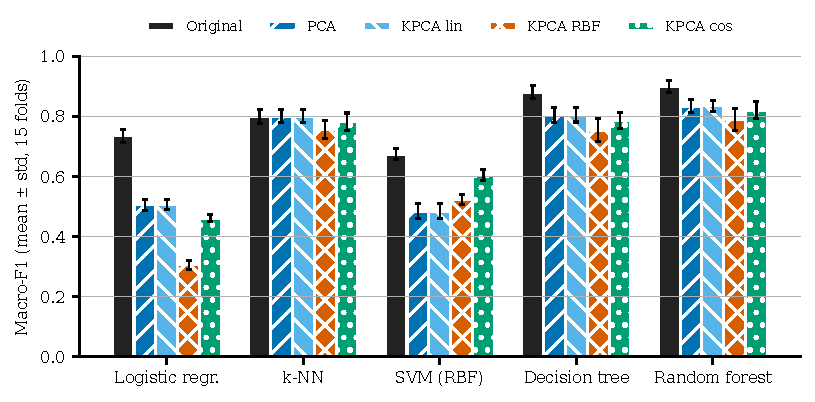
\includegraphics[width=0.68\textwidth]{figures/fig10_all_executions.pdf}
\caption{Macro-F1 of all classifier $\times$ feature-space executions at 10 components (mean $\pm$ std over 15 folds; standard class weights; axis starts at zero).}\label{fig:all}
\end{figure}

\subsection{Accuracy of each algorithm across feature spaces}
Fig.~\ref{fig:peralgo} shows one panel per classifier: bars give mean accuracy for PCA and the three KPCA kernels at 5 to 30 components, and the dashed line is the accuracy on the original 78 features. For logistic regression, $k$-NN, decision tree and random forest, none of the 20 reduced configurations exceeds the original accuracy (the closest is $k$-NN with cosine KPCA at 30 components: 0.9339 against 0.9341). Only the SVM has reduced configurations above its original 0.906, and only cosine KPCA at 15, 20 and 30 components (best 0.924). Accuracy differences are small compared with class-level differences, which is why we use macro-F1 as the primary metric.
\begin{figure}[htbp]\centering
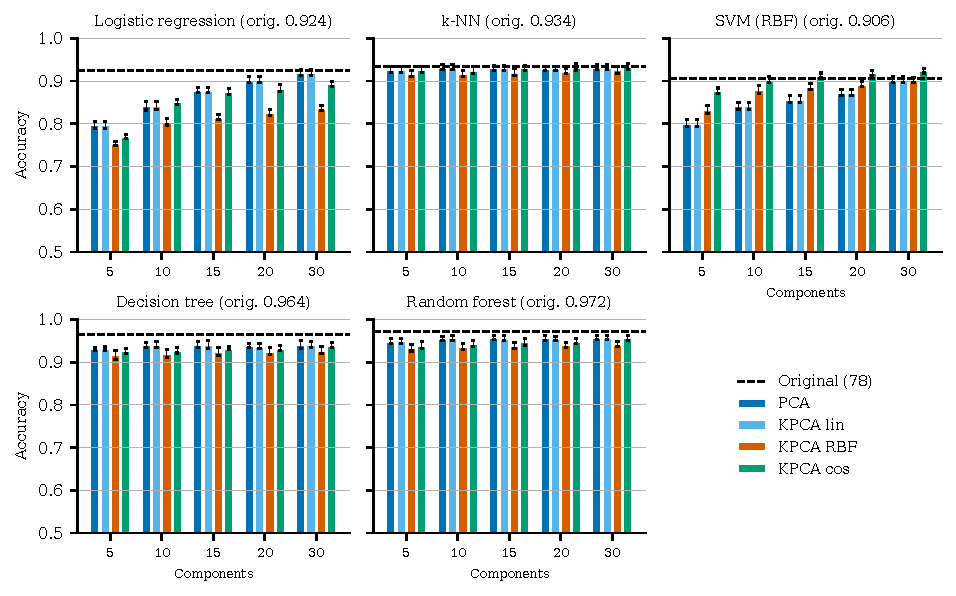
\includegraphics[width=0.84\textwidth]{figures/fig12_per_algorithm_accuracy.pdf}
\caption{Accuracy (mean $\pm$ std over 15 folds, standard class weights) of each classifier for PCA and KPCA at 5--30 components. Dashed line: original 78 features. The vertical axis starts at 0.5.}\label{fig:peralgo}
\end{figure}

\subsection{Selection optimism: nested cross-validation}\label{sec:results-nested}
Selecting the best of 189 configurations on the scoring folds is optimistic, so selection was repeated inside a nested cross-validation (Section~\ref{sec:method}). The configuration chosen on inner folds reached macro-F1 $0.900\pm0.022$ (accuracy 0.972, MCC 0.947) on the outer folds against 0.901 for the same-CV maximum: an optimism of about 0.001. The inner folds chose an original-feature configuration in all 15 outer folds (RF 11 times, DT 4). Original features were clearly better than the inner-selected best reduced space for DT ($+0.093$) and RF ($+0.062$), practically equal for logistic regression ($+0.004$, unadjusted $p=0.010$, far below the fold standard deviation of 0.022) and $k$-NN ($+0.002$), and worse for the SVM ($-0.060$; cosine KPCA-30 chosen in all 15 folds). The $p$-values are unadjusted Wilcoxon tests over 15 outer folds that share training data.



\subsection{Effect of hyper-parameter tuning}
Table~\ref{tab:tuning} reports the nested search (five outer folds). Tuning barely changed the random forest (original 0.901 default, 0.899 tuned; best reduced 0.842 versus 0.839). For $k$-NN it added $+0.007$ on original features, and the gap to the best reduced space stayed within 0.003: 0.000 under defaults (cosine KPCA-30), $-0.002$ after tuning (PCA-30), and $+0.003$ for PCA-30 under defaults. All of these are far below the fold variation. The SVM changed most. Tuned macro-F1 rose from 0.668 to 0.791 on original features and from 0.745 to 0.812 with cosine KPCA-30, so the advantage of reduction shrank from 0.076 to 0.021. Five outer folds cannot establish a difference of 0.021, and the selected values sit on grid edges ($C=10$ for the SVM and $k=3$ for $k$-NN in all 20 selections). We therefore read the SVM advantage of KPCA as a property of the default RBF-SVM that largely disappears with tuning, not as a robust benefit of KPCA.

\begin{table}[htbp]
\caption{Nested hyper-parameter search: mean macro-F1 over five outer folds. For each setting (default, tuned) the best reduced space among PCA-30, KPCA-cos-30 and KPCA-RBF-30 is chosen by that setting\textquoteright s own score; $\Delta$ = original $-$ reduced (negative: reduction better). K-cos-30 = KPCA, cosine kernel, 30 components. The last column gives the default-setting gap measured in the tuned-best reduced space.}\label{tab:tuning}
\centering\scriptsize
\resizebox{\textwidth}{!}{\begin{tabular}{lccrccrr}
\toprule
 & \multicolumn{3}{c}{Default settings} & \multicolumn{3}{c}{Tuned (nested search)} & \\
\cmidrule(lr){2-4}\cmidrule(lr){5-7}
Clf & Orig. & Best reduced & $\Delta$ & Orig.  & Best reduced  & $\Delta$  & $\Delta$ def., tuned-best space \\
\midrule
KNN & 0.801 & 0.801 (K-cos-30) & +0.000 & 0.808 & 0.810 (PCA-30) & -0.002 & +0.003 \\
SVM & 0.668 & 0.745 (K-cos-30) & -0.076 & 0.791 & 0.812 (K-cos-30) & -0.021 & -0.076 \\
RF & 0.901 & 0.842 (PCA-30) & +0.059 & 0.899 & 0.839 (PCA-30) & +0.060 & +0.059 \\
\bottomrule
\end{tabular}
}
\end{table}

\subsection{Row-order robustness (proxy chronology)}
In the head/tail split 4{,}199 records train and 1{,}769 test (32 test records of unseen classes were dropped); only seven of the 15 classes occur in both parts, and infiltration has four test records. The random forest on original features scored 0.838 versus 0.948 for a random split of the same rows and classes (decision tree 0.846 versus 0.959), a penalty of about 0.11. For DT, RF and LR the reduced spaces lost at least as much (RF: PCA-10 0.759, cosine KPCA-30 0.704), so the order original $>$ reduced for DT, RF and LR was preserved; $k$-NN stayed a near tie (0.790 versus 0.806) and the SVM again favoured cosine KPCA-30 (0.616 versus 0.479). In the blocked cross-validation (6--10 classes scored per fold) the random forest scored 0.851 versus 0.932 for random folds on the same classes, with the original space again ahead for DT, RF and LR. Both checks assume that row order follows capture time and score only a subset of classes, so they support the ranking but give no precise penalty.





\subsection{Kernel, component count and class weighting}
Linear KPCA reproduced PCA, as expected on centred data: results were identical for $k$-NN and SVM and within 0.001 (LR) or 0.007 (trees; small eigen-solver differences, not investigated). For LR and SVM the number of components mattered more than the kernel (LR macro-F1 rose from 0.37 at 5 PCA components to 0.73 at 30, against 0.736 on original features). For $k$-NN, DT and RF the kernel mattered somewhat more, but the effects were small. RBF-KPCA with default $\gamma$ was weakest for LR, $k$-NN, DT and RF. For the SVM cosine KPCA was best (mean macro-F1 0.657 versus 0.536 linear and 0.515 RBF; $\gamma$ untuned). Balanced class weights raised balanced accuracy for LR and SVM but macro-F1 only for SVM and DT; they lowered it for LR (0.736 $\to$ 0.710) and RF (0.901 $\to$ 0.885), so the best model remained the unweighted random forest.

\subsection{Computational cost}
The serial benchmark (table in the repository) used 4{,}800 training and 1{,}200 test records. KPCA fitting took 5.5--5.6\,s against 0.02\,s for PCA, more than 200 times as long. It raised decision-tree training from 0.07\,s with PCA to 5.3--5.6\,s and random-forest training from 0.84--0.90\,s to 6.3--6.6\,s, and made random-forest inference about five times slower (0.092--0.123\,s against 0.020--0.021\,s per 1{,}200 records). Peak traced memory of the whole pipeline was 363\,MB for KPCA against 9.8\,MB for PCA or no reduction, about 37 times. It grew roughly quadratically with $n$ (3.1, 11.0, 41.6, 161.3 and 359.1\,MB for $n=400$ to $4800$; log--log slope 1.9), consistent with an $n\times n$ float64 kernel matrix (184\,MB at $n=4800$). As arithmetic, not a measurement, one dense float64 kernel matrix for all 2{,}830{,}743 source flows would need about 64\,TB, so exact KPCA on the full dataset would require approximation or sub-sampling (not tested).







\subsection{Accuracy comparison with recent studies}
Fig.~\ref{fig:cmp} and Table~\ref{tab:lit} put reported accuracies side by side. The values in Table~\ref{tab:lit} range from 97.75\,\% to 99.9965\,\%, and Fig.~\ref{fig:cmp} plots 99.987\,\% for Emirmahmuto\u{g}lu and Atay, the lower of their two stated values; our random forest reaches 97.2\,\% accuracy but 0.901 macro-F1 on a sample that over-represents attacks. These figures are not comparable. They illustrate only that a high accuracy says little about minority-class detection: ours is 0.972 with web-attack F1 of 0.53 and 0.59.


\begin{figure}[htbp]\centering
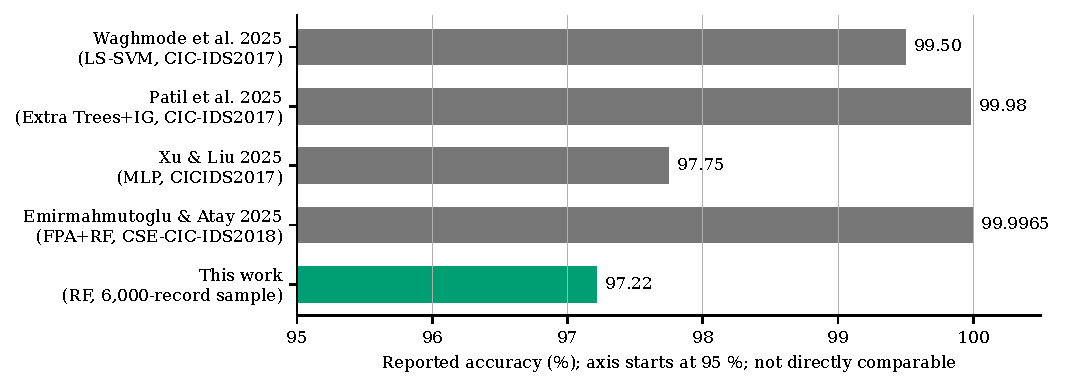
\includegraphics[width=0.85\textwidth]{figures/fig11_accuracy_comparison.pdf}
\caption{Accuracy reported by recent studies versus this work (lower of the two values given by Emirmahmuto\u{g}lu and Atay is plotted). The horizontal axis starts at 95\,\%. Datasets, sample designs, splits and metrics differ, so the bars are not a like-for-like ranking.}\label{fig:cmp}
\end{figure}

\section{Discussion}
\textbf{Answers to the research questions.} RQ1 and RQ2: reducing the 78 standardised features to 5--30 PCA or KPCA components mostly did not help and usually lowered macro-F1. The loss was clear for the decision tree and random forest and negligible for logistic regression (30 components) and $k$-NN. The one gain, the RBF-SVM with cosine KPCA, largely disappeared under tuning (0.076 to 0.021). RQ3: for $k$-NN, DT and RF the kernel mattered slightly more than the number of components; for LR and SVM it was the other way round. Default-$\gamma$ RBF was weakest for four of five classifiers, and linear KPCA equals PCA. RQ4: at $n=4{,}800$, KPCA multiplied reducer fit time by more than 200 and traced memory by about 37 (memory grows quadratically), with no benefit for four of five classifiers. RQ5: orderings were stable across repeated folds, nested selection, tuning and the scorable row-order splits.

\textbf{Why accuracy misleads.} Benign flows make up 67.2\,\% of the sample, so a classifier that always says ``benign'' already scores 0.672. The best model's 0.972 accuracy sits alongside web-attack F1 of only 0.53 and 0.59.

\textbf{Possible explanations (untested).} We ran no experiment to separate the following hypotheses. (i) Trees split on one feature at a time, so rotating the data into principal components may hide axis-aligned thresholds (on packet or flag counts, for example) that trees can exploit; this would fit the clear losses for DT and RF. (ii) PCA keeps the directions of largest variance, and these need not be the directions that separate rare classes such as the web attacks. (iii) For the SVM, a default RBF kernel with $\gamma=$ ``scale'' on 78 standardised features may be poorly matched to the data. The gain from cosine KPCA fell from 0.076 to 0.021 once $C$ and $\gamma$ were tuned, which is consistent with this but does not prove it.

\section{Threats to Validity and Limitations}
The conclusions should be read with the following limitations in mind.

\textbf{1. Sample, not full data.} All results come from \emph{one} stratified sample of 6{,}000 records out of 2.5\,M de-duplicated flows (0.24\,\%), because exact KPCA is quadratic in memory. The sample has a floor of 100 records per class and is \emph{not} prevalence-preserving: attack classes are over-represented, so accuracy, macro-F1 and class priors do not describe deployment-time prevalence. Heartbleed (11 records), SQL injection (21) and infiltration (36) are complete but tiny, so their per-class estimates are very uncertain, and another random sample could change rankings that differ by a few points. We did not repeat the pipeline over several sampling seeds.

\textbf{2. Leakage status.} Sampling was performed on the raw, un-imputed data, and imputation, scaling and reduction are fitted inside each training fold. Remaining possible leakage channels were \emph{not} eliminated: records from the same attack session or burst can still fall into both training and test folds in the random 5-fold design, and near-duplicate (not exact-duplicate) flows are not removed. The row-order checks reduce but do not remove this concern, and they rest on the unproven assumption that row order follows capture time.

\textbf{3. Limited external validity.} All data come from one dataset captured in one testbed over one week. The row-order checks score only seven classes (head/tail split) or six to ten classes per fold (blocked) and use a single split or five folds; there is no cross-dataset evaluation. These conclusions hold only for random and within-file row-ordered splits of CIC-IDS2017, not for drift over real time.

\textbf{4. Selection and inference.} The headline configuration (RF, original features) was the best of 189 on the same cross-validation that produced its score. The nested analysis shows the optimism is about 0.001 macro-F1 here, but the nested estimate itself is conditioned on the same sample. Repeated-CV significance tests violate independence \cite{nadeau2003}; $p$-values are screening evidence, and unadjusted values are reported for the nested comparisons.

\textbf{5. Limited tuning.} Hyper-parameter search covered only $k$-NN, SVM and random forest, four spaces and five outer folds, with small grids whose optimum lay on the edge for $k$-NN and SVM $C$. Logistic regression, the decision tree and the KPCA kernel parameters ($\gamma$ for RBF) were not tuned, so conclusions about those are about default settings. Class weighting was the only imbalance treatment; resampling was not evaluated.

\textbf{6. Dataset quality and cost.} The original CIC-IDS2017 flows contain known labelling and feature-construction artefacts \cite{engelen2021}, which may distort scores (and may explain the web brute-force/XSS confusion); we did not use the corrected release. Timings and memory come from one shared 2-vCPU virtual machine, memory is a traced lower bound, and differences below about a factor of two should not be over-interpreted; we make no real-time claim.



We propose no new algorithm and make no claim of state-of-the-art, real-time or production-ready performance, or of generalization beyond this sample. The finding we can support is narrower: on this sample, original features were at least as good as PCA or KPCA for four of five classifiers, the one exception largely vanished with tuning, and accuracy hid a systematic failure on web attacks.

\section{Conclusion}
We set out to learn whether PCA or KPCA improves intrusion detection over the 78 original CIC-IDS2017 features. On a class-stratified sample of 6{,}000 records, it mostly did not. A random forest on the original features scored highest (macro-F1 $0.901\pm0.020$; accuracy $0.972\pm0.004$; $0.900\pm0.022$ with nested selection). Reduction to 5--30 components was clearly worse for the decision tree and random forest, and at best practically equal for logistic regression (30 components) and $k$-NN (RQ1, RQ2). Only the RBF-SVM benefited, from cosine KPCA, and that advantage shrank from 0.076 to 0.021 after tuning. Linear KPCA coincided with PCA, and for LR and SVM the number of components mattered more than the kernel (RQ3). At 4{,}800 records KPCA needed more than 200 times the reducer fit time of PCA and about 37 times the traced memory (RQ4). The ranking held across repeated folds, nested selection, tuning and the two row-order checks, which assume without proof that row order follows capture time (RQ5). Accuracy hid weak detection of web brute force and XSS (F1 0.53 and 0.59). These findings apply only to this sample of CIC-IDS2017.

\textbf{Future work.} Repeat the pipeline over several sampling seeds and larger samples with an approximate KPCA; add cross-dataset evaluation; widen the tuning grids and tune the KPCA kernel parameters; test the corrected CIC-IDS2017 release \cite{engelen2021}; and evaluate session-grouped splits.


\section*{Data and Code Availability}
The raw CIC-IDS2017 MachineLearningCVE files are distributed by the dataset provider \cite{sharafaldin2018} and are not redistributed here. The sampling script, the sampling manifest (file names, raw and de-duplicated class counts, seed), all experiment, analysis and claim-checking code, per-fold raw results and the generated tables and figures are available at \ifdefined\BLIND a repository whose link is withheld for anonymous review\else[REPOSITORY URL / ARCHIVE DOI - TO BE FILLED BY THE AUTHORS]\fi.


\section*{Acknowledgments and AI-assistance disclosure}
Generative AI was used in this work. Claude (Anthropic; Claude Code, model Claude Sonnet 5.5) helped (i) write and revise the Python pipeline (data preparation, cross-validation, nested CV, tuning, row-order checks, statistics, runtime benchmark, tables, figures and an automated claim checker); (ii) draft and edit the text of all sections, including the abstract, captions and limitations; and (iii) look up and cross-check bibliographic metadata and statements attributed to cited sources. ChatGPT (OpenAI) was used for editorial suggestions and for additional checks of cited sources. All reported numbers were produced by code run on the data described and re-checked by script. The authors reviewed the content and remain fully responsible for it. The authors received no specific funding for this work and declare no competing interests.

\bibliographystyle{splncs04}
\bibliography{references}
\end{document}
